\date{15 января 2025}

\section{Связность}

\subsection{Линейная связность}

\begin{definition}
    [Путь]
    В топологическом пространстве $X$ путь из $a\in X$ в $b\in X$ -- это непрервыное отображение $\alpha\colon [0,1]\to X$, т.ч. $$\alpha(0) = a, \quad\alpha(1)=b.$$ 
\end{definition}

\begin{definition}
    [Линейная связность]
    Пространство $X$ линейно связно, если \[\forall a,b\in X \quad \exists\text{путь из }a \text{ в }b.\]
\end{definition}

\begin{theorem}
    Пусть $X, Y$ -- топологические пространства, $X$ линейно связно, $f\colon X\to Y$ непрерывное. Тогда $f(X) \subset Y$ тоже линейно связно. 
\end{theorem}
\begin{proof}
    Любые две точки из $f(X)$ нужно соединить путём. Но такие точки имеют вид $f(a), f(b)$. Тогда возьмём путь $\alpha\colon[0,1]\to X$, соединяющий $a$ с $b$. Тогда $(f\circ \alpha)\colon[0,1]\to f(X)$ тоже является путём, соединяющий $f(a)$ с $f(b)$.
\end{proof}
\begin{corollary}
    Если $X\underset{homeo}{\cong} Y$ и $X$ линейно связно, то $Y$ тоже линейно связно.
\end{corollary}

Дальш будет пример доказательства \emph{не} гомеоморфности двух пространств.

\begin{example}
    Пусть $X = (0;1), Y = (0;1) \cup (1;2)$. Тогда $X$ и $Y$ не гомеоморфны. 
    
    Ведь $X$ линейно связно: путь из $a \in (0;1)$ в $b \in (0;1)$. Тогда можно взять путь $\alpha(t) = (1-t)a+tb$ -- равномерное прямолинейное движение. А $Y$ не линейно связно, т.к. из точки $\frac 1 2$ в точку $\frac 3 2$ нет пути, т.к. нет такой непрерывной функции по теореме о промежуточном значении.
\end{example}

\subsubsection{Компоненты линейной связности}

\begin{theorem}
    В топологическом пространстве $X$ можно ввести отношение эквивалентности $\sim$, где $a\sim b$, если существует путь из $a$ в $b$.
\end{theorem}
\begin{proof}
    \begin{conditions}
        \item \emph{рефлексивность}: $\alpha(t) = a$ -- путь из $a$ в себя.
        \item \emph{симметричность}: если $\alpha$ путь из $a$ в $b$, то возьмём \begin{equation}
            \beta(t) \coloneq \alpha(1-t).
        \end{equation}
        \item \emph{транзитивность}: если $\alpha$ путь из $a$ в $b$, $\beta$ путь из $b$ в $c$, то возьмём путь из $a$ в $c$ \begin{equation}
                \gamma(t) \coloneq \begin{cases}
                \alpha(2t), &t\in[0;\rfrac 1 2];\\
                \beta(2t), &t\in[\rfrac 1 2; 1].
            \end{cases}
        \end{equation}
    \end{conditions}
\end{proof}

\begin{definition}[Компоненты линейной связности]
    Классы эквивалентности называется компонентами линейной связности пространства $X$. $$\pi_0(X) = \{\text{компоненты линейной связности}\}.$$
\end{definition}

\begin{example}
    $X$ -- дискретная топология. Тогда компоненты -- точки.
\end{example}

\begin{proposition}
    Если $A \subset \R^n$ выпукло, т.е. $$[a; b]\defeq \{(1-t)a+tv\such t\in[0;1]\}\subset A.$$ То $A$ линейно связно.
\end{proposition}

\begin{example}
    $[0; 1]$ и $[0;1]^2$ не гомеоморфны. 

    Пусть $h\colon[0;1] \to [0;1]^2$ гомеоморфизм. Тогда \begin{equation}
        h\colon[0;\rfrac 12]\cup[\rfrac 1 2; 1]\to [0;1]^2 \setminus \{h(\rfrac 1 2)\}.
    \end{equation} тоже гомеоморфизм. Но $[0;\rfrac 12]\cup[\rfrac 1 2; 1]$ не линейно связно, а $[0;1]^2 \setminus \{h(\rfrac 1 2)\}$ линейно связно, т.к. мы всё еще можем построить хорошие пути (\cref{fig:square-proof}).
\begin{figure}[h]
    \centering
    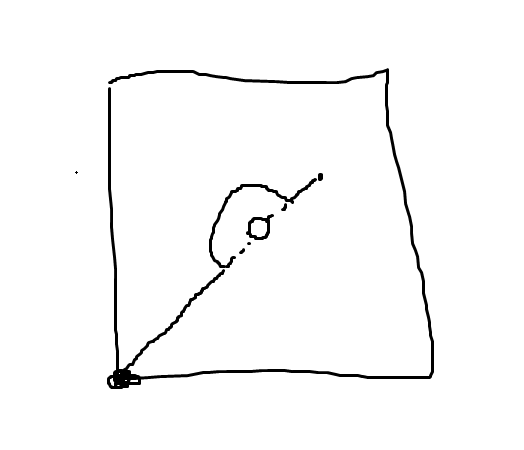
\includegraphics[width=0.5\linewidth]{graphics/square-proof.png}
    \caption{Квадрат всегда можно повернуть, так чтобы выделенная вершина была левая нижняя.}
    \label{fig:square-proof}
\end{figure}
\end{example}

\subsection{Связность}

\begin{example}
    $X = \{(x,\sin x)\such x>0\}\cup\{0\}\times[-1,1]$. 
    \begin{figure}[ht]
        \centering
        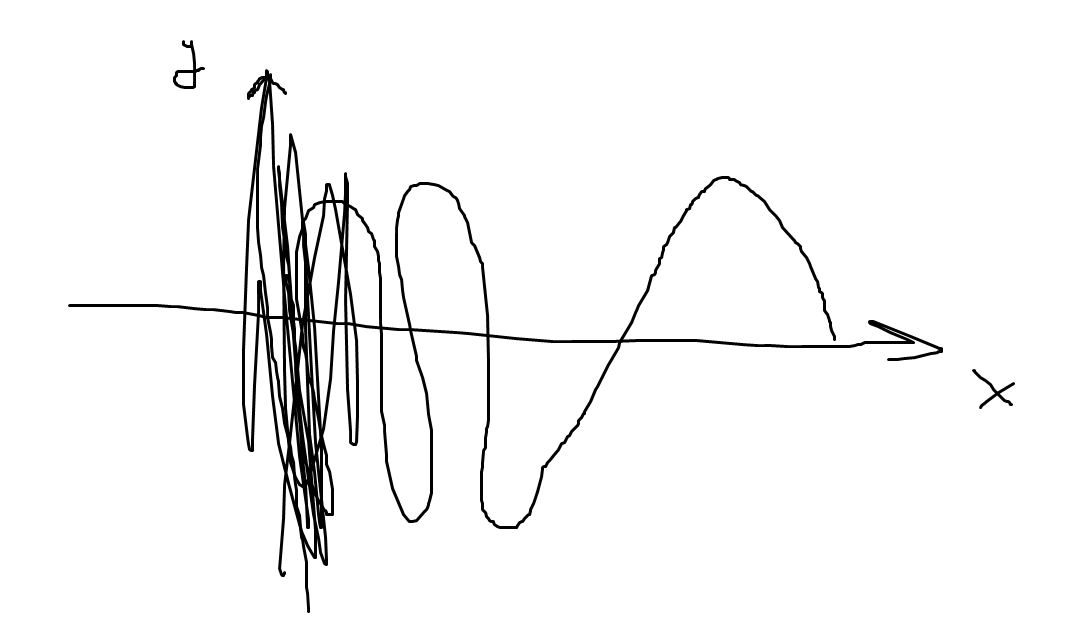
\includegraphics[width=0.75\linewidth]{graphics/sinx_x-graph.png}
        \caption{График множества $X$.}
    \end{figure}

    Но не существует пути в $X$ из $(0,0)$ в $\left(\frac 1 \pi; 0\right).$

    Пусть путь $\alpha(t)$ существует, тогда \(\alpha(t) = (u(t), v(t))\), где $u, v$ -- непрерывные функции. Причем $t\to 0\implies \alpha(t) \to (0,0).$ Тогда по теореме о промежуточном значении \begin{equation}
        \exists (t_n)_{n\in\N}\to 0, \quad u(t_n) = \frac{2}{(4n+1)\pi} 
    \end{equation}для больших $n$. \begin{equation}
        v(t_n) = \sin{\frac 1 {u(t_n)} = \sin{\frac{\pi}{2}} (4n+1)} =1 \not\to 0.
    \end{equation}
\end{example}

\begin{definition}
    [Связность]
    Пространство $X$ \emph{не} связно, если выполнено одно из эквивалентных условий: \begin{conditions}
        \item $X = A \cup B, \quad A\cap B = \varnothing, \quad A, B\neq\varnothing, \quad A, B \in \T_X.$
        \item $X = A \cup B, \quad A\cap B = \varnothing, \quad A, B\neq\varnothing, \quad A, B \text{ замкнуты}.$
        \item Существует нетривиальное $(\neq 0, X)$ открытое и замкнутое множество в $X$.
    \end{conditions}
\end{definition}

\begin{theorem}
    $X$ связно, $f\colon X \to Y$ непрерывно, тогда $f(X)$ связно.
\end{theorem}
\begin{proof}
    Рассмотрим $\phi\in H^0(X, \R)$. Тогда $\phi \circ f \in H^0(X, \R)$, а значит $\phi\circ f = const.$, а значит и $\phi = const.$
\end{proof}

\begin{theorem}
    $[0; 1]$ связен 
\end{theorem}
\begin{proof}
    Пусть он не связен, т.е. можно представить в виде объединение открытых непустых и непересекающихся множеств $A, B$. Неформально можно думать, что отрезок покрашен в красные и синие точки (\cref{fig:colored-segment}). 
    \begin{figure}[ht]
        \centering
        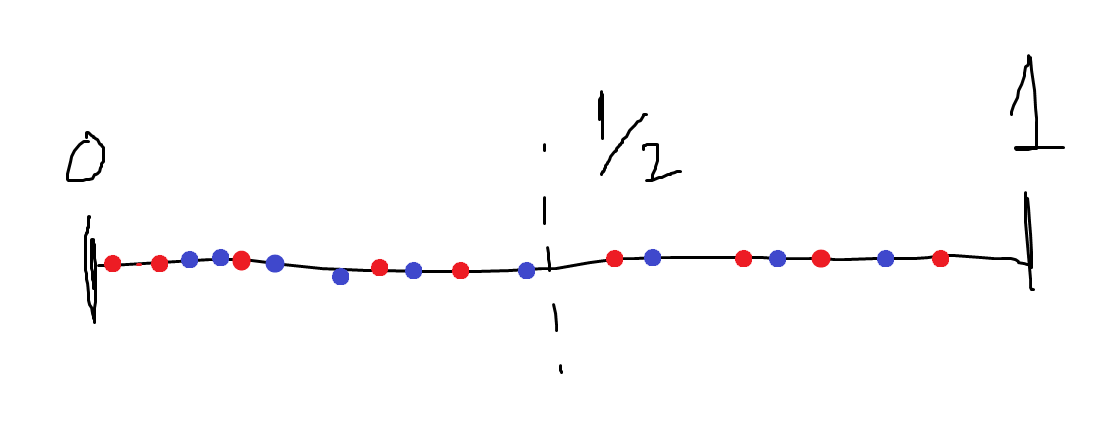
\includegraphics[width=0.75\linewidth]{colored-segment.png}
        \caption{Наш ``покрашенный'' отрезок}
        \label{fig:colored-segment}
    \end{figure}
    Выберем половину покрашенную в разные цвета ($I_1$) и продолжим этот процесс. Получим \begin{equation}
        [0,1] \supset I_1 \supset I_2 \supset \ldots, \quad \{c\} = \bigcap_{} I_n.
    \end{equation} Пусть $c \in A$ (WLOG). Тогда с одной стороны $(\exists \epsilon > 0) (c-\epsilon; c+\epsilon) \cap [0;1] \subset A.$ А с другой стороны $(\exists n ) I_n \subset (c-\epsilon, c+\epsilon) \cap [0;1].$
\end{proof}

\begin{example}
    Связные множества в $\R$ -- это \emph{только} промежутки $(a,b)$, $[a, b)$, $[a,b]$, $(a,b]$.
\end{example}
\begin{proof}
    Пусть $A \subset \R$ связно, тогда $A$ выпукло, иначе $x < y$ лежит в $A$, а точка $z \in (x;y)$ не лежит в $A$. Но тогда \begin{equation}
        A = \underbrace{(A\cap(-\infty; z))}_{\ni x}\cup\underbrace{(A \cap (z; +\infty))}_{\ni y}. 
    \end{equation}
    Но тогда $A$ несвязно, что неправда. Тогда \begin{equation}
        A = (\underbrace{\inf A}_{=a}, \underbrace{\sup A}_{=b})\cup C, \quad C \subset \{a, b\}.
    \end{equation}
\end{proof}